\section{Architecture}
\label{sec:architecture}

\subsection{Overview}

Figure~\ref{fig_allmodules} depicts the architecture of Vermont.
The functionality is divided into two main modules: A sampler module and a concentrator module.
The sampler module implements all packet-based functions like packet capturing, filtering, sampling and PSAMP export.
The functions for flow accounting and aggregation are provided by the concentrator module.
Both main modules can run independently or in combination; in the second case, the sampled packets are passed from the sampler module to the flow metering and aggregation function of the concentrator module.
A common exporter library called ipfixlolib realizes the export of monitoring data using the IPFIX/PSAMP protocol.

Both main modules are broken up into submodules, which are described in the following subsections.
The main modules, as well as their submodules, have been designed for being instantiated more than once, giving the user a maximum degree of flexibility and caring for a wide range of monitoring needs.
This modular approach also guarantees a high level of re-usability and eases the incorporation of selected components into other software packages.

Vermont's modular design excels where customization is needed.
Implementing the SQL database writer was a matter of simply writing an alternative export module and changing Vermont's configuration routines so it could be instantiated when configured to.
A base class takes care of the details like allocating buffered queues and two methods have to be implemented which start and shutdown the submodule's operation.
We use an URI-based scheme to indicate the export method used, i.e. exporting to the host \texttt{10.20.30.40} with destination port 4739 (standard port assigned to IPFIX) using the UDP protocol is expressed by \texttt{udp://10.20.30.40:4739}. This scheme can be arbitrarily extended.

%Internally, each of Vermont's three main functions - capturing, filtering and exporting - is contained within its own thread.
%Forwarding data between subsystems is done by putting references to the actual data into buffered queues connecting the subsystems.
%This design was chosen to fully exploit multi-processor-systems and, ultimately, aid scalability by allowing asynchronous processing while avoiding unnecessary copying or locking of data.
Internally, submodules are contained within different threads.
In order to avoid unnecessary copying of data, only references to the actual data are passed from one subsystem to the other using buffered queues.
This design was chosen to optimally exploit the asynchronous processing capabilities of multi-processor systems.

Vermont's configuration is maintained in one consistent configuration file, following the XML schema proposed in~\cite{muenz-ipfix-configuration}. In addition, a back-end for dynamic reconfiguration using Netconf protocol has been implemented~\cite{muenz2006using}, allowing for fast remote distribution of new configuration data.

Depending on the configuration, Vermont captures raw packets, performs packet sampling and optional flow accounting, and exports the resulting monitoring data using the IPFIX/PSAMP protocol.
Alternatively, Vermont can operate as an IPFIX concentrator that receives and aggregates data exported by other monitoring probes in order to reduce the overall data volume.


\begin{figure}
\begin{center}
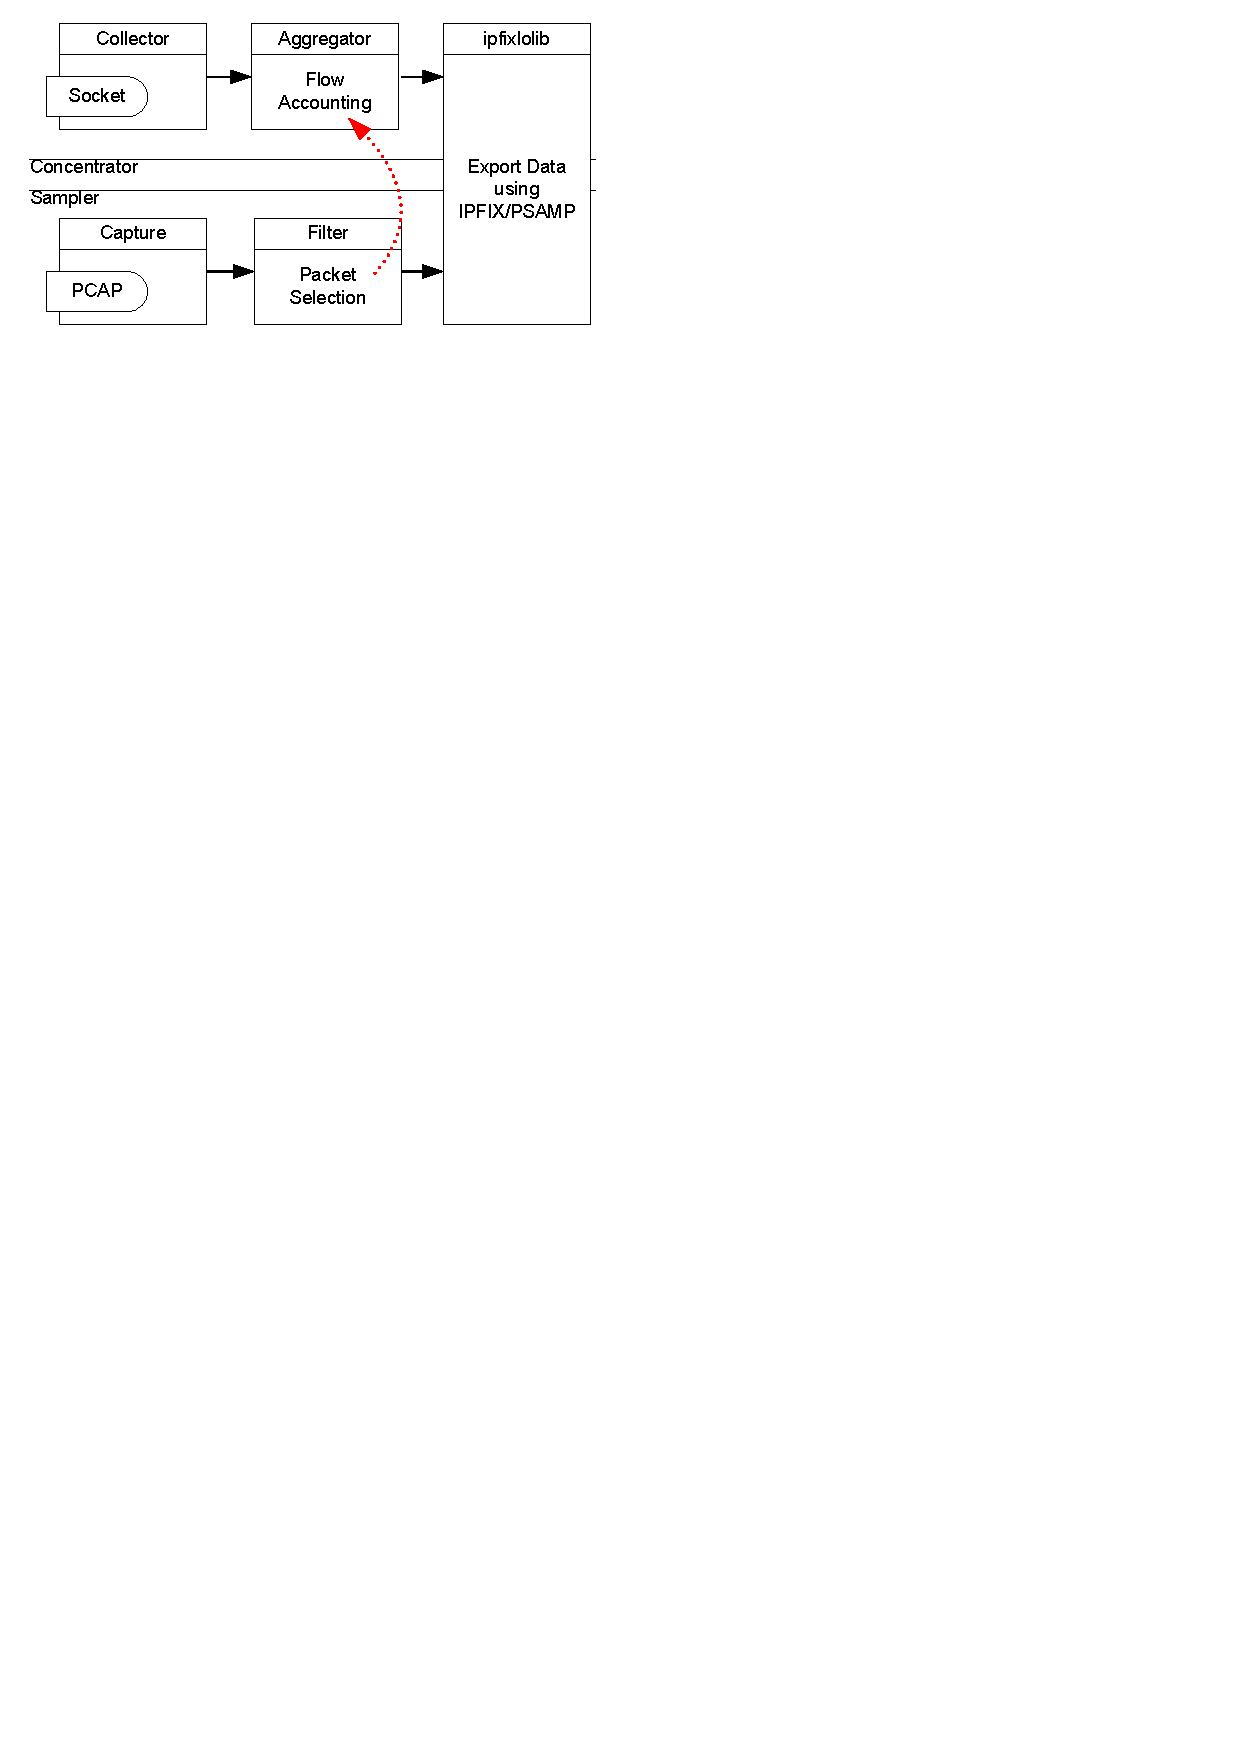
\includegraphics[scale=0.65]{gfx/vermont-arch2.pdf}
\caption{Vermont: Architectural overview}
\label{fig_allmodules}
\end{center}
\end{figure}


\subsection{Sampler Module}
\label{sec_sampler}

The sampler module captures raw packets from network interfaces, selects individual packets based on filters and sampling algorithms as specified in~\cite{ietf-psamp-sample-tech} and exports the resulting data.
Filters and sampling algorithms are implemented as packet processors that can be executed in arbitrary order.
% that provide all fields required by the configured templates
Non-matching packets or packets that are sorted out by a sampling algorithm are immediately dropped and only packets that have passed all packet processors are exported.
At any point in the packet processor chain, packets can also be injected into the concentrator module to be processed by the flow metering and aggregation function.

\subsection{Concentrator Module}
\label{sec_concentrator}

Vermont's concentrator module consists of a NetFlow.v9/IPFIX collector, an aggregator and an IPFIX exporter, all interconnected using callbacks.
The aggregator submodule implements the rule-based flow metering and aggregation approach specified in~\cite{dressler-ipfix-aggregation}.
It can be configured to process flows received via the IPFIX collector and/or packets injected by the sampler module; this is shown in figure~\ref{fig_allmodules} by the dotted arrow.
That way, the aggregator can be deployed for flow accounting of local traffic as well as for concentration of flow records received from other monitoring probes. 


%\subsection{ipfixlolib}
%\label{sec_ipfixlolib}
%
%Both subsystems export their data using a library aiding the sending of IPFIX/PSAMP-encoded data.
%It provides a C API with the following functionalities:
%\begin{itemize}
%\item conversion of IPFIX identifiers into their numerical representation et vice versa
%%\item automatic conversion of data and meta-data from HBO to NBO et vice versa
%\item protocol-compliant periodic export of templates
%\item export of metering data to one or several collectors
%\end{itemize}


\section{Monitoring Scenarios}
\label{sec:scenarios}

% "some of which" sounds really nice -RLA
Owing to the flexibility offered by its modular design, Vermont can be used in a wide range of scenarios, some of which are presented in this section. Data export can be done to one or more collecting stations.

\subsection{PSAMP Probe}
With only the sampler module activated, Vermont acts as a PSAMP probe that captures packets from network interfaces, selects individual packets based on filters and sampling algorithms and exports the resulting packet-based monitoring data.

\subsection{IPFIX Probe}
In this mode, Vermont performs rule-based flow accounting~\cite{dressler-ipfix-aggregation} on locally observed packets. Both the sampler module and the concentrator module are activated.
The sampler module is configured to pass packets to the concentrator module, which performs flow accounting and exports the resulting flow records. For example, flow accounting can be used to generate byte or packet counters for the observed network.
The sampler module's exporter, as well as the concentrator module's collector, are disabled.

\subsection{Concentrator}
Only the concentrator module is activated. Flow records from other monitoring probes are received at the collector. Rule-based flow aggregation~\cite{dressler-ipfix-aggregation} is performed in order to reduce the amount of monitoring data.
The resulting records are exported to higher-level concentrators or traffic analyzers.

\subsection{Specific accounting for SYN flood detection}
In the context of \emph{Diadem Firewall}, Vermont is used to count TCP SYN and SYN/ACK packets. The resulting counter values are used to detect SYN flood attacks on protected servers using the SYN-dog algorithm~\cite{wang02syndog}.

